%!TEX root = ../my_thesis.tex
\section{The LHCb experiment}
\label{sec:lhcb}

The \emph{Large Hadron Collider beauty} (LHCb) experiment~\cite{LHCb-DP-2014-002} is a single-arm forward spectrometer (see Fig.~\ref{fig:detector}) that exploits the forward production
of the $b$- and $c$- quark pairs in $pp$ collisions (Fig.~\ref{fig:angles}). The LHCb angular coverage is comprised between $15~\rm mrad$ and $250$ ($300$) $\rm mrad$ in the vertical (horizontal) plane.
The LHCb coordinate system consists of a right-handed set of axes, $x$, $y$, $z$, where the positive $z$ direction extends into the LHCb detector, $y$ is perpendicular to the LHCb cavern ground and $x$ is orthogonal to the other two.

\begin{figure}[htbp]
  \begin{center}
    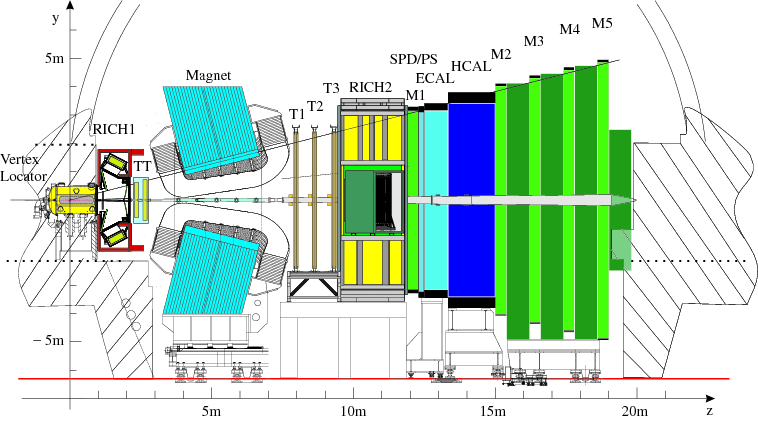
\includegraphics[width=0.9\textwidth]{02LHCb/figs/detector.png}
  \end{center}
  \vspace{-2mm}
  \caption{Side view of the LHCb detector.}
  \label{fig:detector}
\end{figure}

The LHCb experiment is composed of different sub-detectors. The tracking system includes a vertex and tracking detector called \emph{VErtex LOcator} (VELO), the \emph{Tracker Turicensis} (TT), located upstream a magnetic dipole with an integrated field of $4~\rm Tm$, the \emph{Inner Tracker} (IT), situated downstream the magnet in three separated stations around the beryllium beam pipe, and the \emph{Outer Tracker} (OT), installed in the same stations as the IT. The \emph{Particle IDentification} (PID) system comprises two \emph{Ring Imaging CHerenkov} detectors (RICH), an \emph{Electromagnetic CALorimeter} (ECAL), which also includes a \emph{Pre-Shower} (PS) and \emph{Scintillator Pad Detector} (SPD), a \emph{Hadronic CALorimeter} (HCAL) and five \emph{muon stations} (M1--M5).

\begin{figure}[htbp]
  \begin{center}
    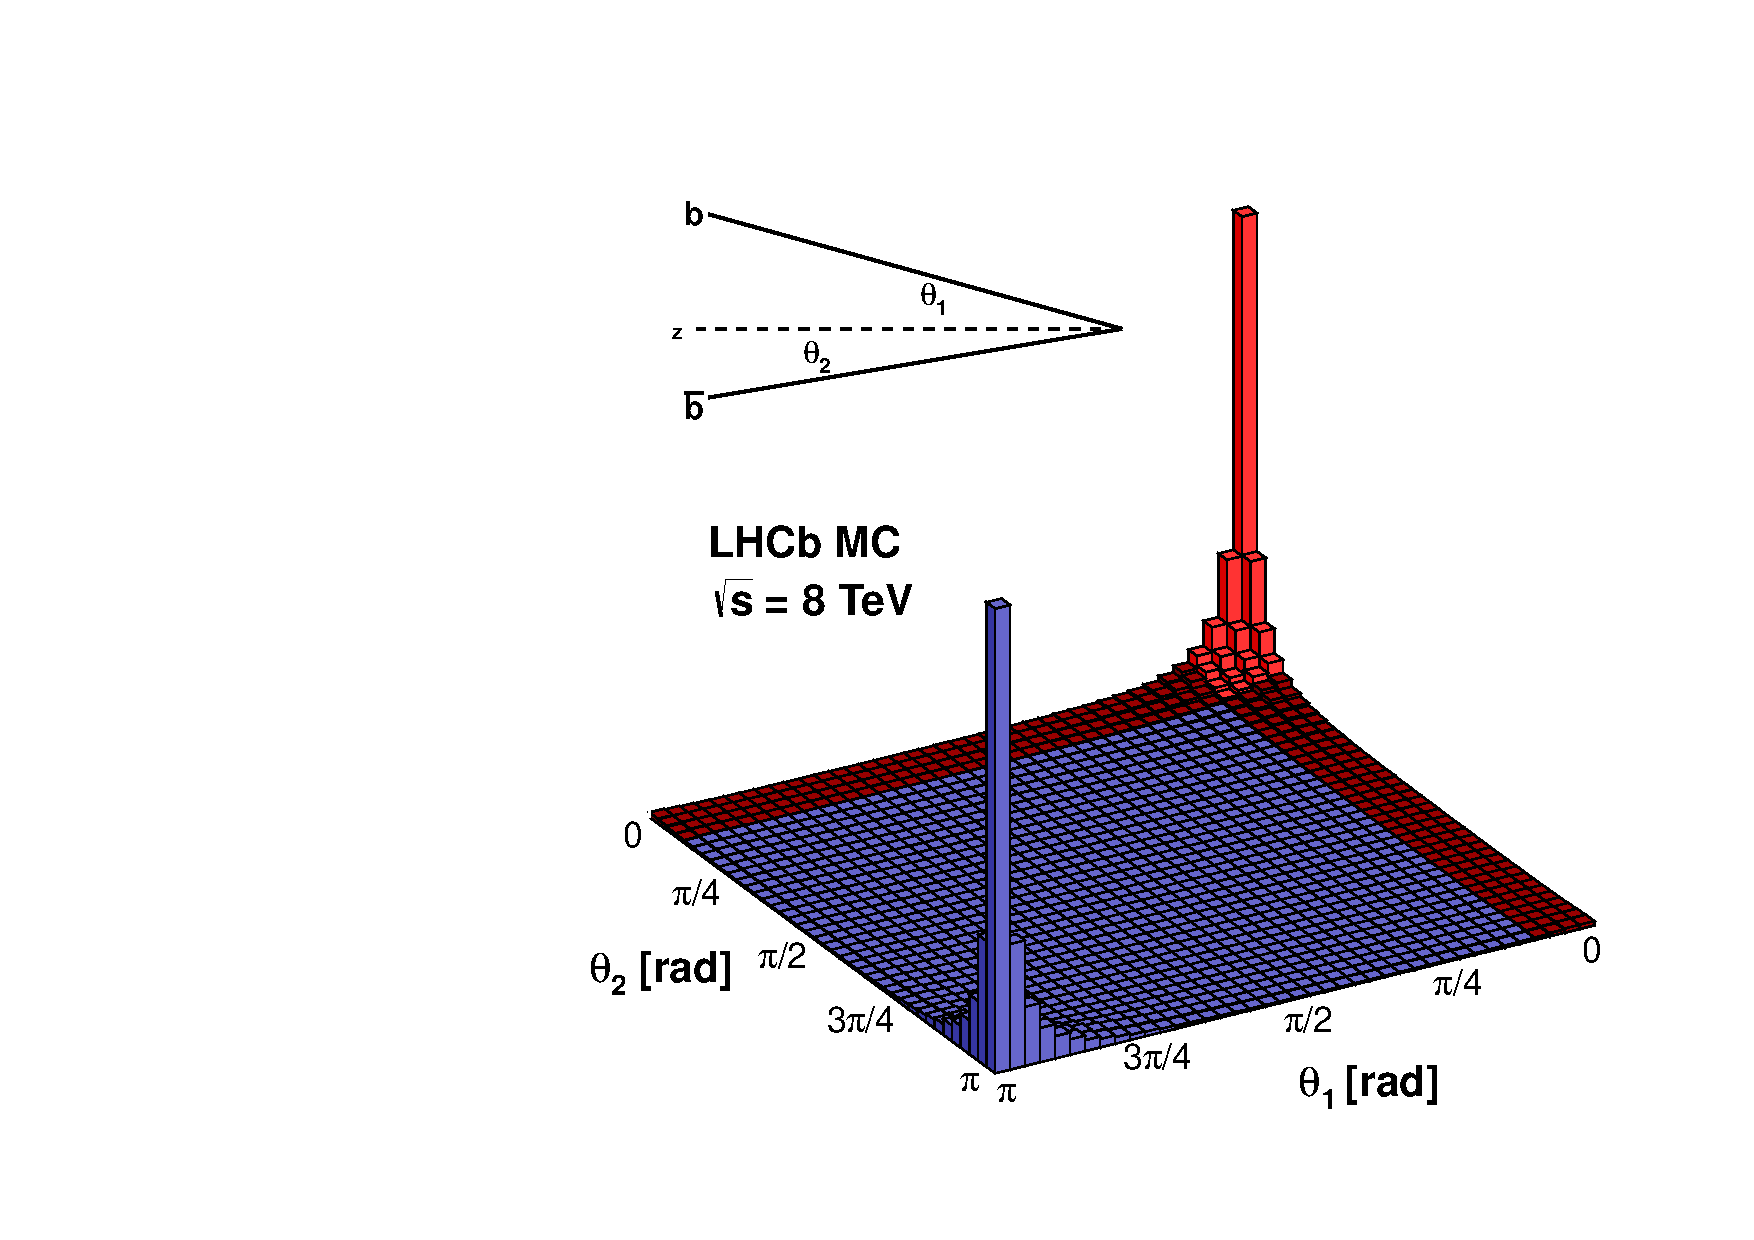
\includegraphics[width=0.5\textwidth]{02LHCb/figs/angles.pdf}
  \end{center}
  \vspace{-2mm}
  \caption{Joint distribution of the $b$ and $\bar b$ production angles with respect to the beam direction at $\sqrt{s}=8\rm~TeV$, as obtained from simulation. The red part shows the LHCb acceptance.}
  \label{fig:angles}
\end{figure}

\subsection{Tracking system}
\label{sec:tracking}

The tracking system plays a crucial role for the time-dependent analysis of $\Bz\to\Dmp\pip$ decays at LHCb.
The excellent vertex and impact-parameter resolution allows to separate true, long-lived $\Bz$ mesons from combinations of
other random tracks, and to improve the decay-time resolution.
Moreover, the optimal momentum resolution implies an excellent resolution on the reconstructed invariant mass, which is crucial
to separate true $\Bz\to\Dmp\pip$ decays from other physical background.

The tracking system is also essential for the flavour tagging algorithms, which rely on the quality of the reconstructed tracks and
vertices to discriminate correctly tagged neutral $B$ mesons from wrongly tagged ones.

A summary of the performances of the tracking system (momentum, impact-parameter, and decay-time resolution) is shown in Fig.~\ref{fig:track_perf}.

\begin{figure}[htbp]
  \begin{center}
    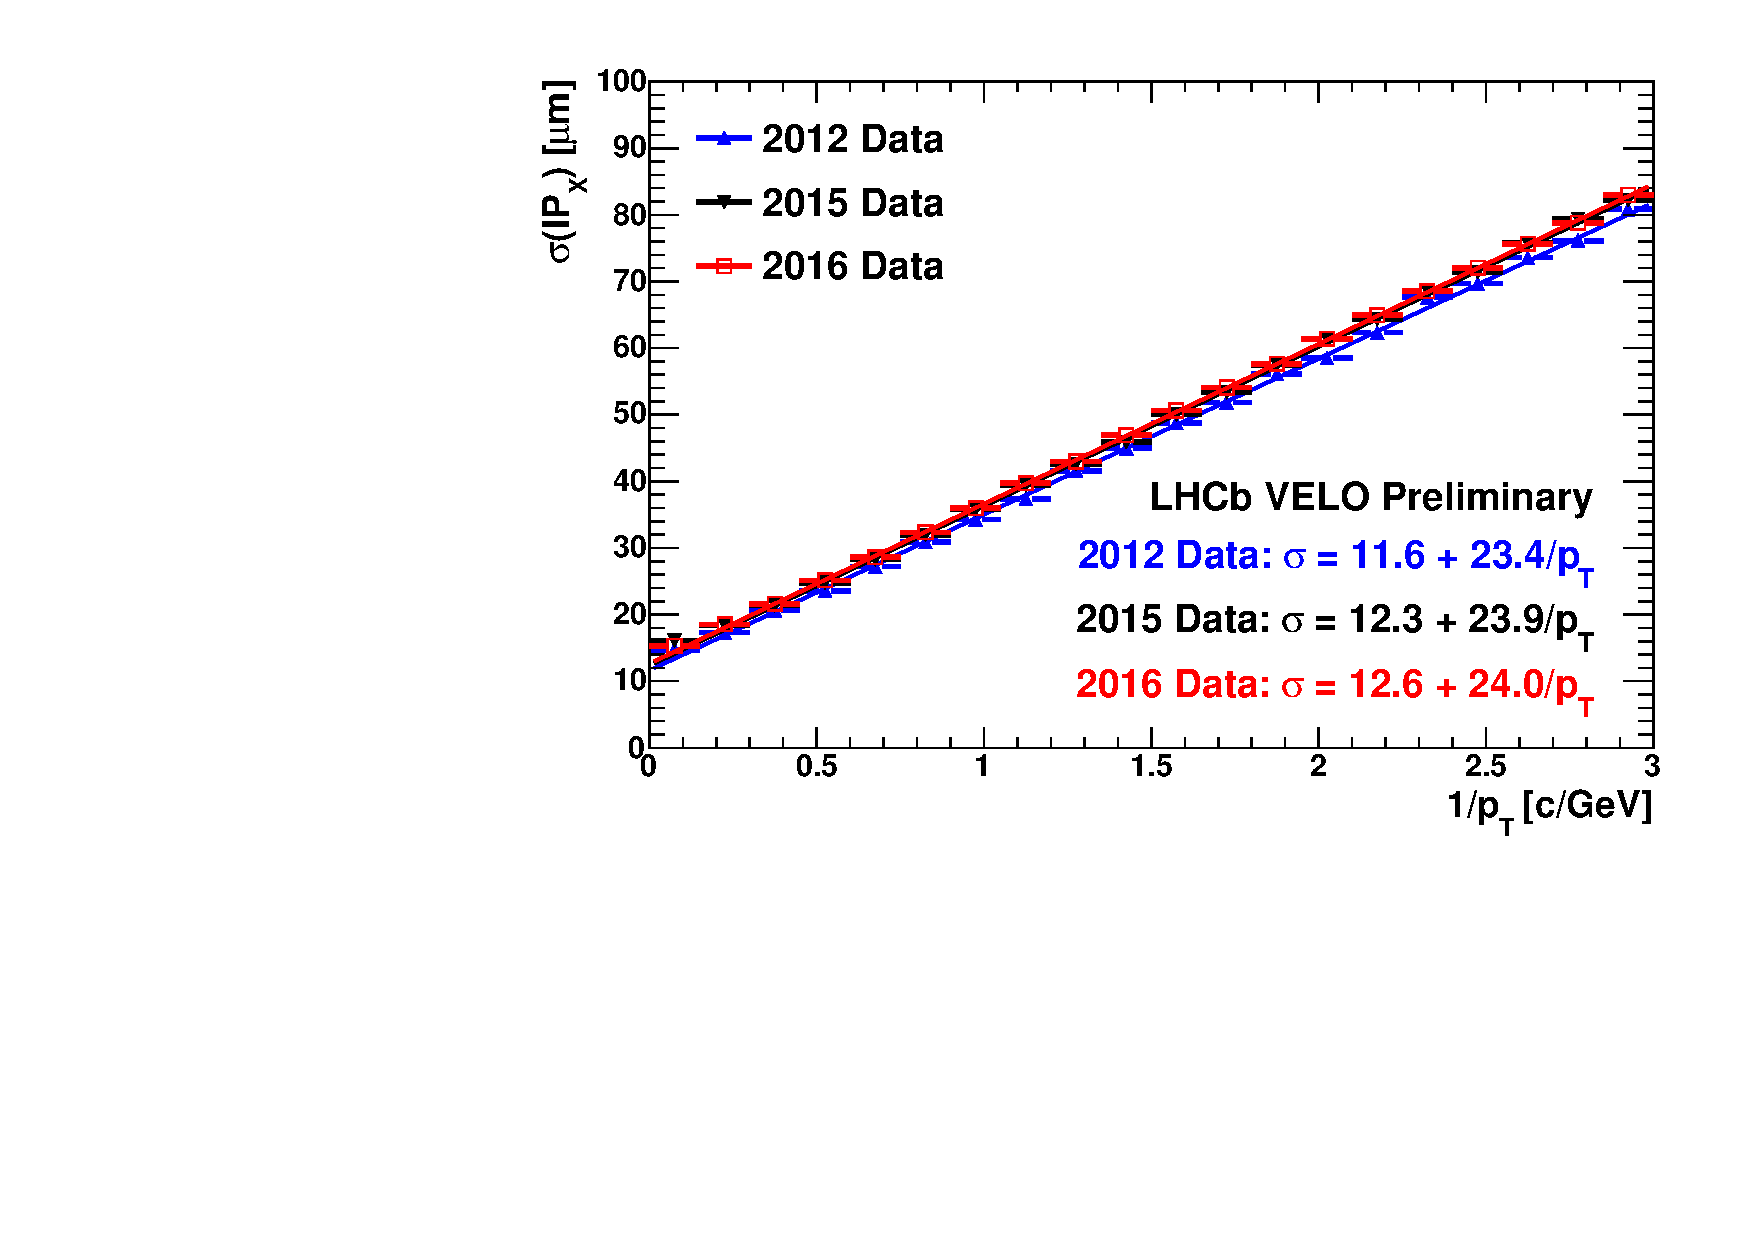
\includegraphics[width=0.48\textwidth]{02LHCb/figs/IPX-resolution.pdf}
    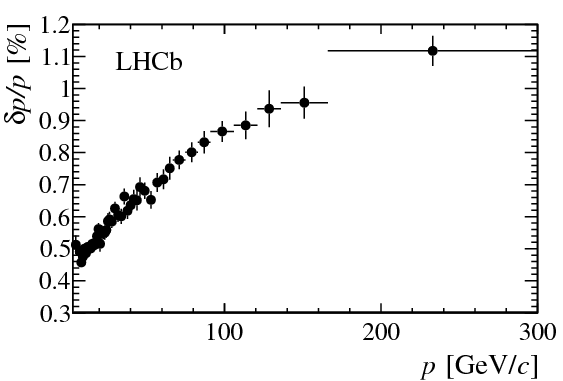
\includegraphics[width=0.48\textwidth]{02LHCb/figs/momentum_resolution.png} \\
    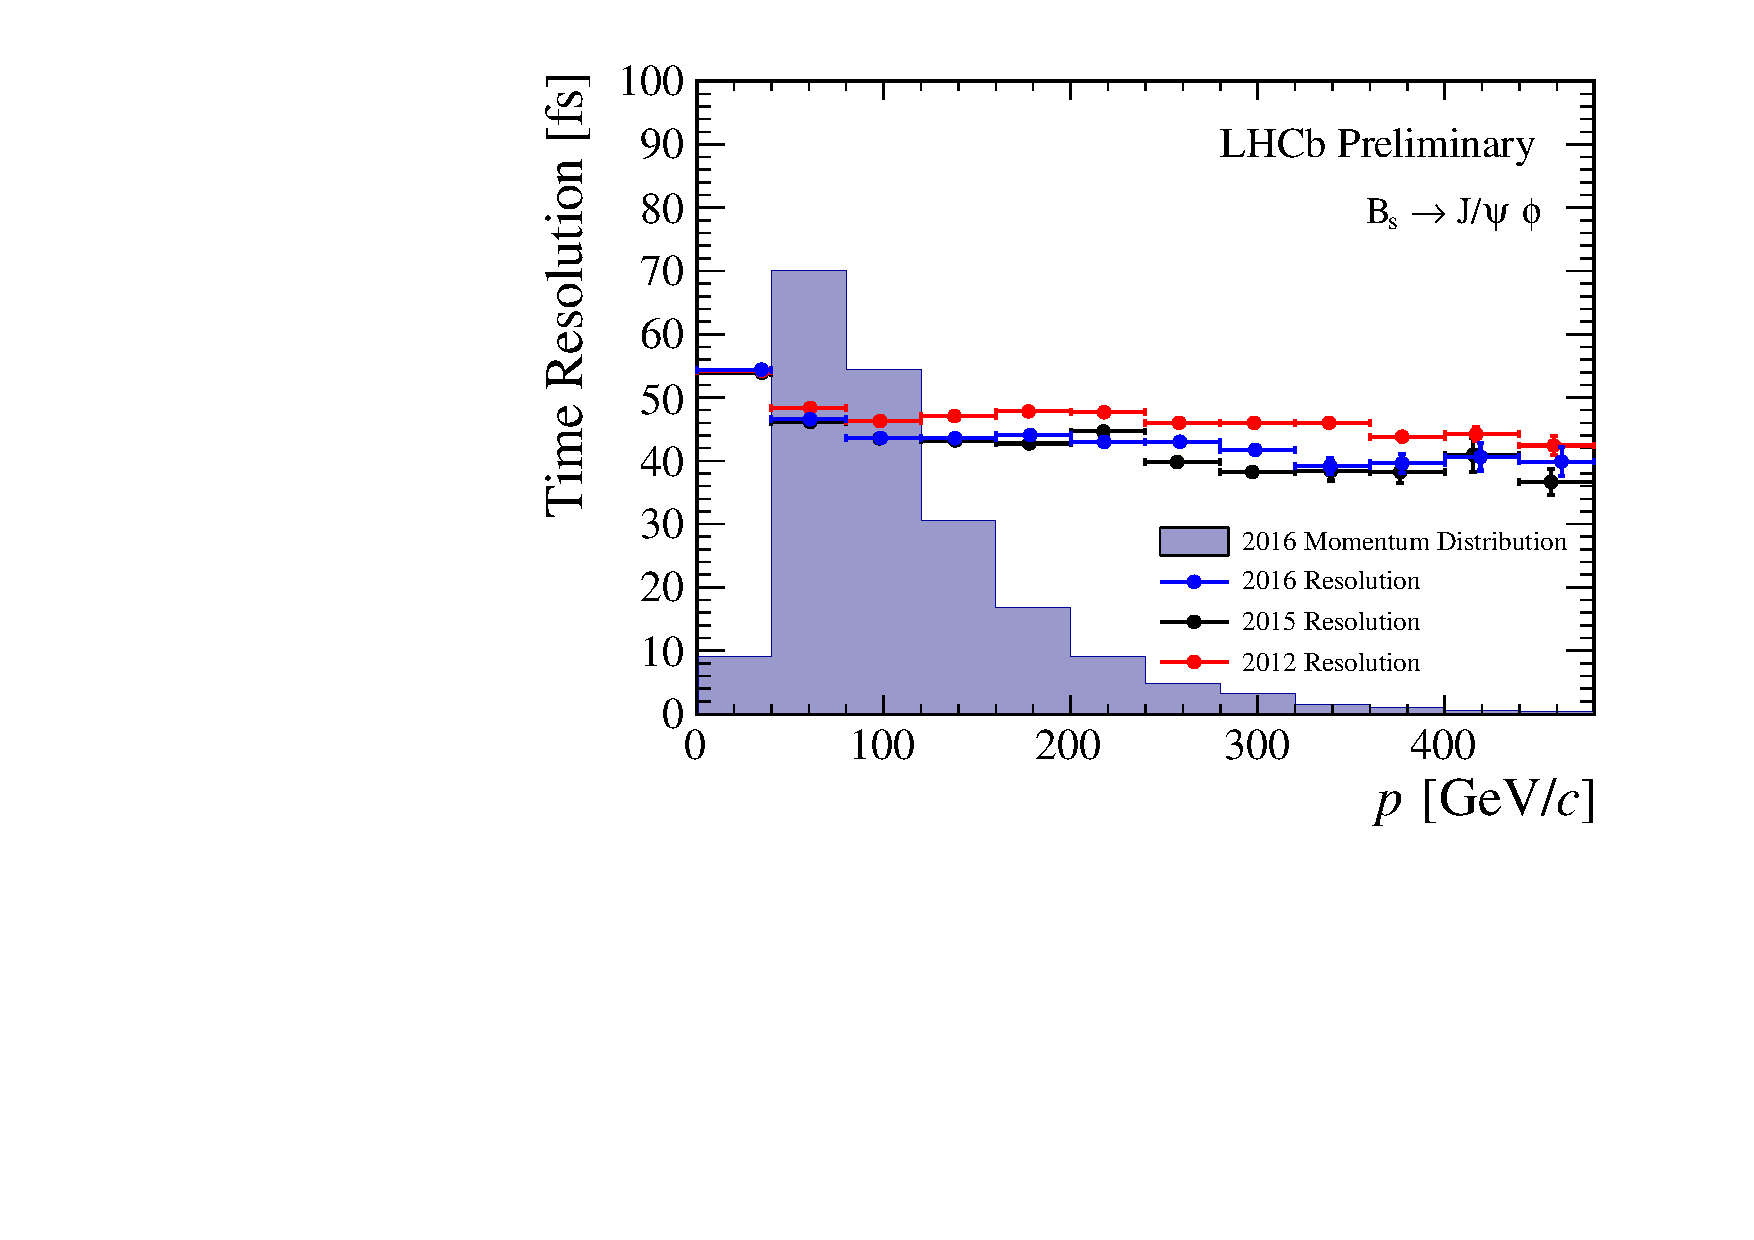
\includegraphics[width=0.48\textwidth]{02LHCb/figs/decay_time_res.pdf}
    \vspace{-5mm}
  \end{center}
  \caption{Top left: resolution on the $x$ coordinate of the impact parameter as a function of the inverse of the reconstructed transverse momentum in
  2012 (blue), 2015 (black) and 2016 (red) data. The result of a linear fit for each dataset is superimposed.
  Top right: relative momentum resolution as a function of the reconstructed momentum.
  Bottom: decay-time resolution as a function of momentum for reconstructed $\Bs\to J/\psi\phi$ decays in 2012 (red), 2015 (black) and
  2016 (blue) data. The momentum distribution is superimposed as the solid, purple histogram.}
  \label{fig:track_perf}
\end{figure}

\subsubsection*{The VErtex LOcator (VELO)}

The VELO \cite{LHCb-DP-2014-001} (Fig.~\ref{fig:VELO}) is a silicon micro-strip detector surrounding the interaction point, which detects charged particles, performs the first track reconstruction step and identifies decay vertices.
The sensitive region of the VELO is composed of n-on-n silicon micro-strip half-disk sensors with two different read-out strip geometries, called $r$-type and $\phi$-type, which measure the radial ($r$) and azimuthal ($\phi$)  position in polar coordinates. The silicon sensors are $8.4~\rm cm$ in diameter and have an inner hole with radius $0.8~\rm cm$. The strip pitch ranges from $38$ to $108~\rm\mu m$ ($38$ to $97~\rm\mu m$) for $r$ ($\phi$) sensors, while the sensor thickness is $300~\rm\mu m$.
The VELO consists of 21 stations placed perpendicular to the beam axis. Each station has two independent halves that can be moved apart during beam injection and then closed again when the beam orbit is stabilised. Each half-station is composed by one $r$-type and one $\phi$-type sensor. The total length of the VELO detector is about $1~\rm m$.
The impact parameter (IP) resolution of a track is measured to be $\sigma_{\rm IP}=11.6\pm23.4/\pt~\rm\mu m$ in $x$ and  $\sigma_{\rm IP}=11.2\pm23.2/\pt~\rm\mu m$ in $y$, where $\pt$ is the \emph{transverse momentum} (in $\gevc$) of the particle with respect to the beam axis. 

\begin{figure}[t]
  \begin{center}
    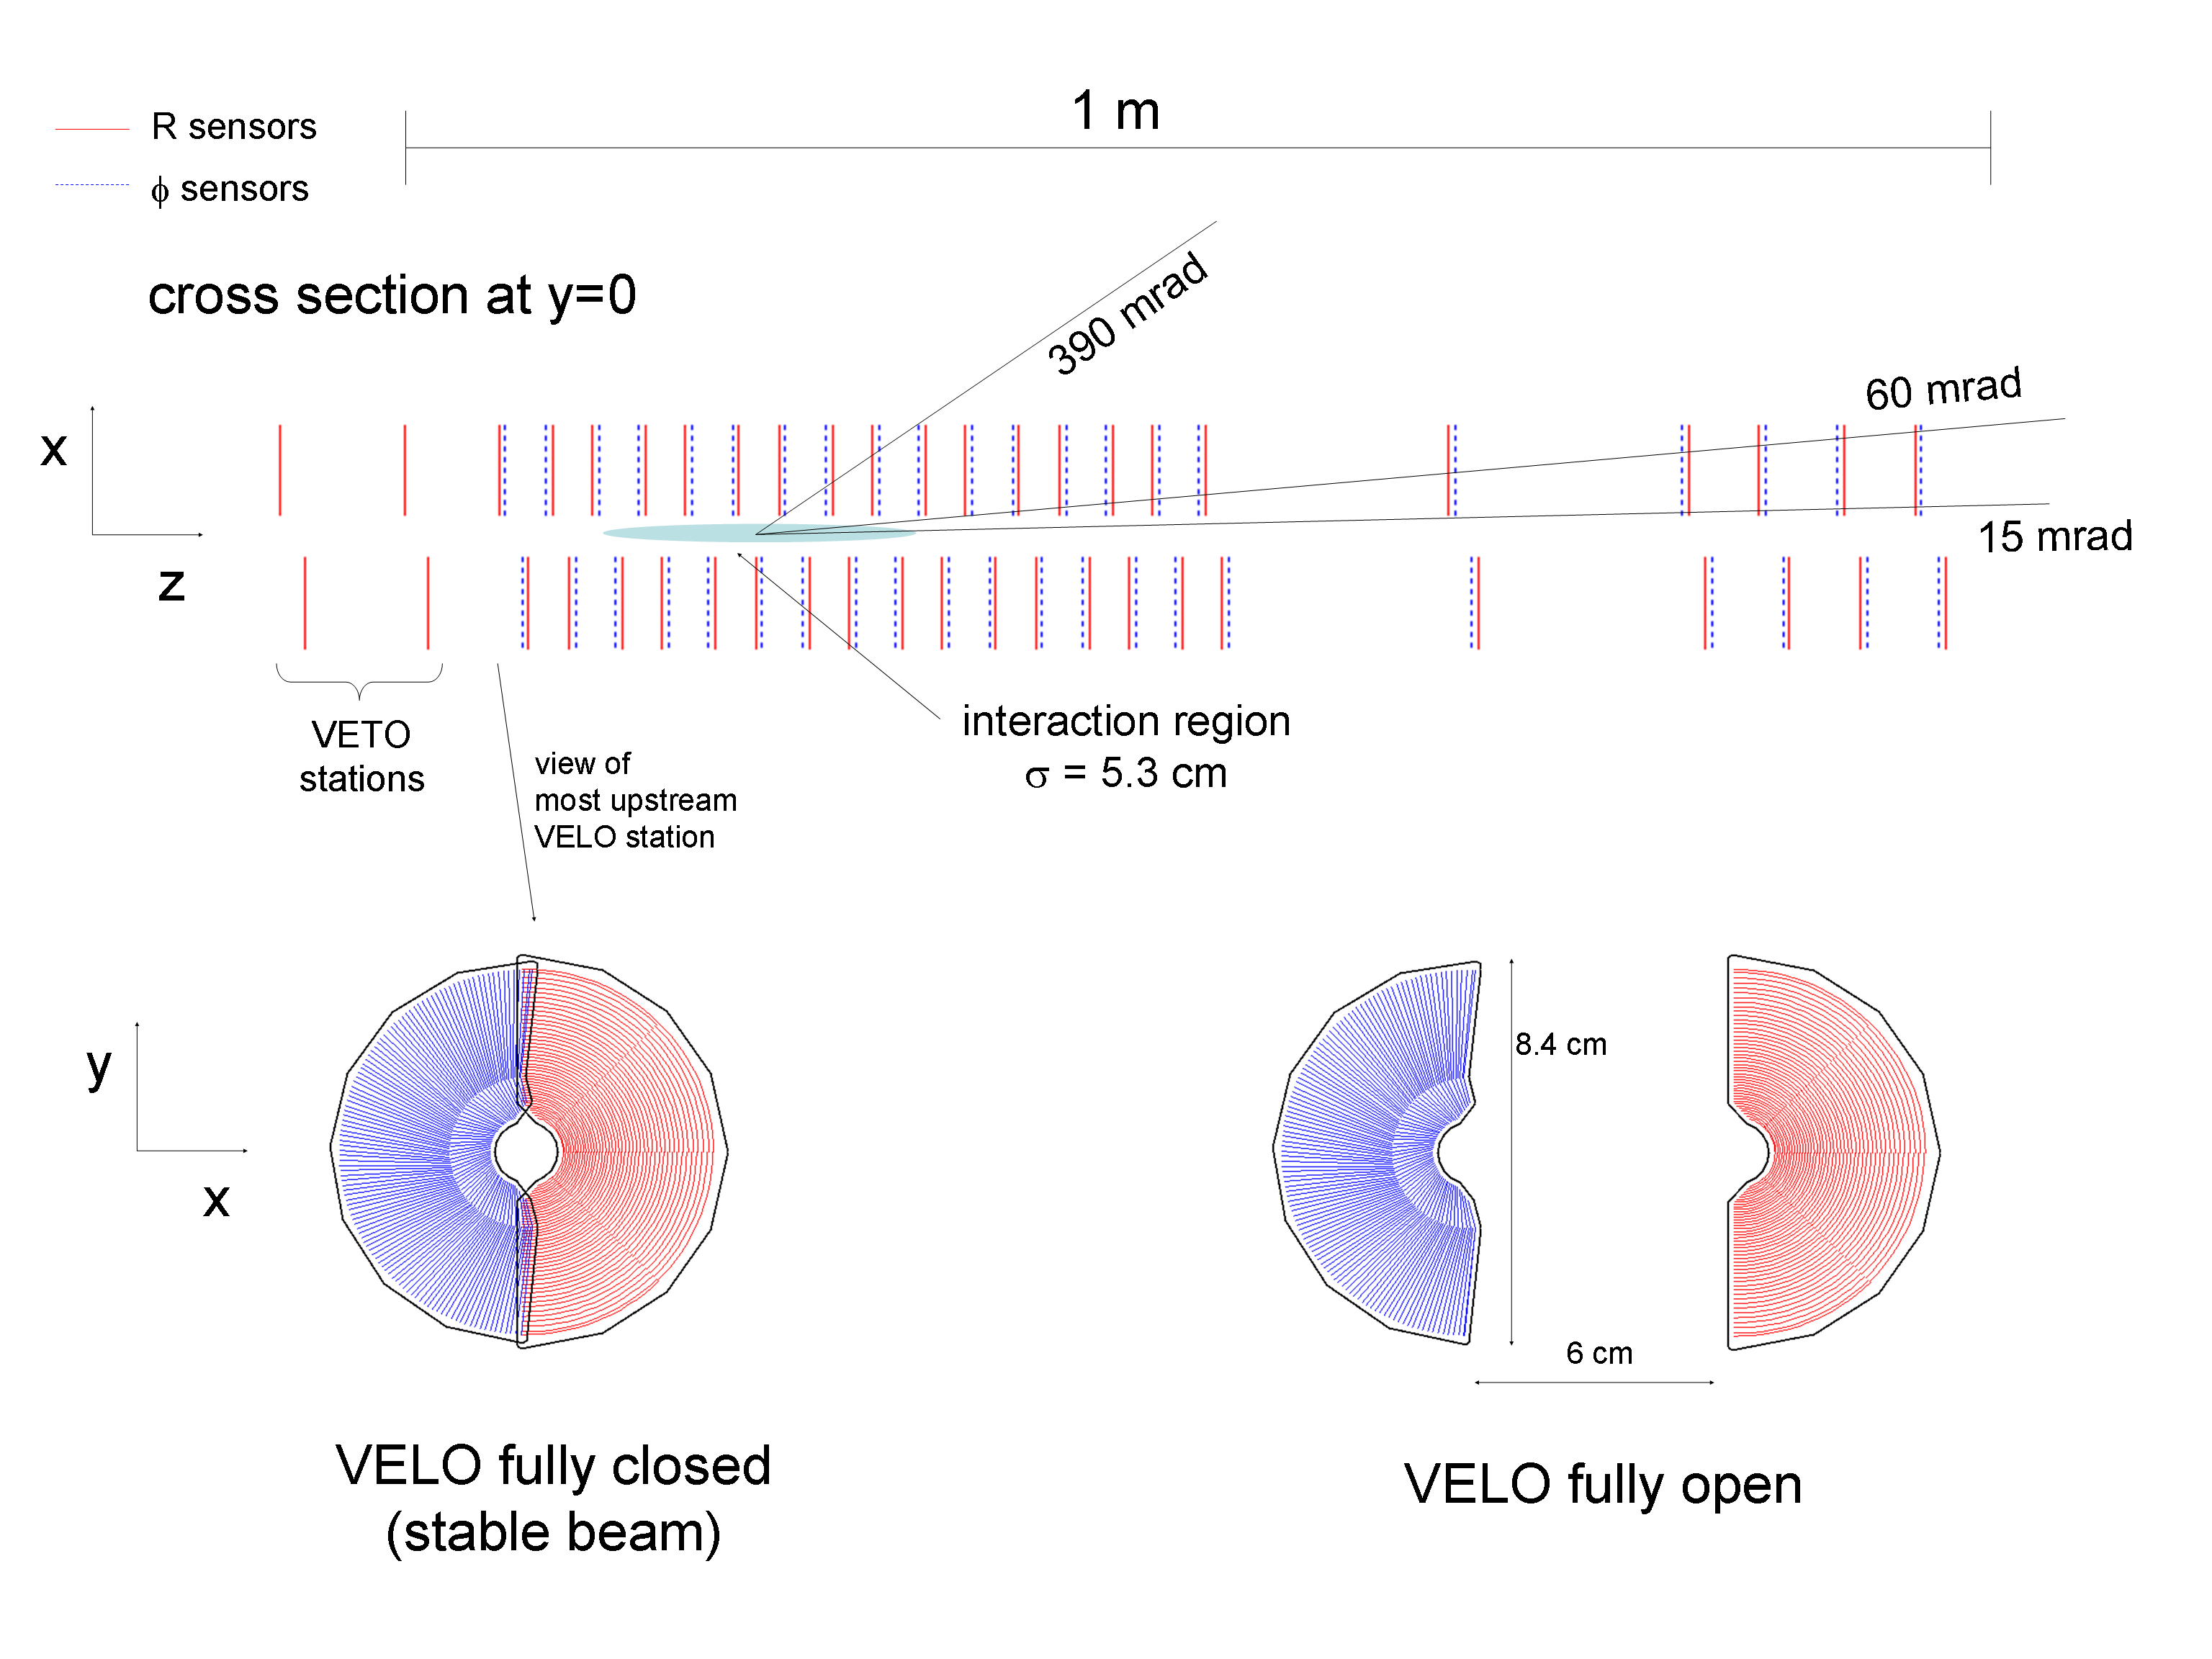
\includegraphics[width=0.9\textwidth]{02LHCb/figs/velo.png}
  \end{center}
  \vspace{-2mm}
  \caption{Schematic view of the VELO detector (top) and its sensors (bottom).}
  \label{fig:VELO}
\end{figure}

\subsubsection*{The Tracker Turicensis (TT)}

The TT \cite{LHCb-TDR-009} (Fig.~\ref{fig:TT}) is a silicon micro-strip detector covering a total area of about $7.9~\rm m^2$ upstream the magnet and divided into two separate stations (TTa, TTb). Each station has two layers. The TT helps in improving the track momentum resolution and detecting long-lived particles that decay outside the VELO acceptance. TTa is composed of a X and an U layer, while TTb includes a V and an X layer. The X layers have readout strips aligned vertically, whereas the U and V \emph{stereo} layers are rotated by $+5^{\degree}$ and $-5^{\degree}$ with respect to the vertical in the $xy$ plane.

\begin{figure}[t]
  \begin{center}
    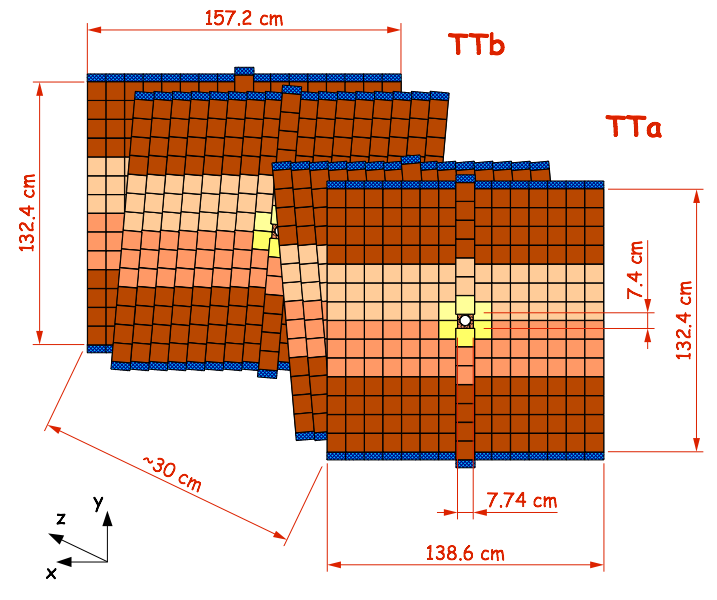
\includegraphics[width=0.4\textwidth]{02LHCb/figs/TT-scheme.png}
    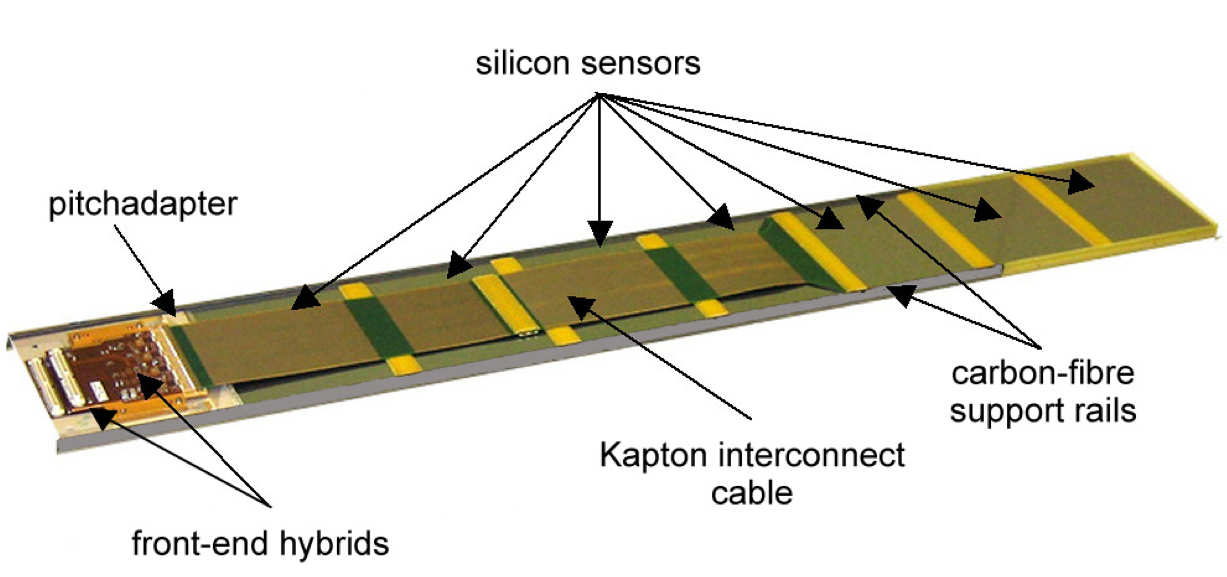
\includegraphics[width=0.4\textwidth]{02LHCb/figs/TT-strip-layout.png}
  \end{center}
  \vspace{-2mm}
  \caption{Schematic view of the TT stations/layers (left) and one of the TT readout modules (right).}
  \label{fig:TT}
\end{figure}


The TT active area is made of p-on-n silicon micro-strip sensors. Since the sensors are exposed to a significant radiation dose due to the high track multiplicity, they are cooled to $0^{\degree}$C in order to minimise the effect of reverse annealing due to radiation damage.

A TT readout module contains from one to four sensors connected in series, resulting in read-out strips up to $37~\rm cm$ long. The strip pitch is $183~\rm\mu m$ and the sensor thickness is $500~\mu m$. The hit resolution is about $50~\mu m$.

\subsubsection*{The Inner Tracker (IT)}

The IT \cite{LHCb-TDR-008} (Fig.~\ref{fig:IT}) is also a silicon micro-strip detector. Together with the TT, it forms the \emph{Silicon Tracker} (ST). It is dedicated to detect charged particles in the high track-density region around the beam pipe downstream the magnet. It is separated into three stations, where each station consists of four boxes. Each box has four layers made of seven read out modules arranged in a X-U-V-X layout similar to that of the TT.
The total coverage of the IT is about $4.2~\rm m^2$. The boxes directly above and below the beam pipe are made of single-sensor modules, called \emph{short modules}, whereas the side boxes are made of two bonded silicon sensor modules, called \emph{long modules}. The IT strip pitch is $198~\rm\mu m$, while the p-on-n sensor thickness is $320$ ($410$) $\mu m$ for the short (long) modules. The hit resolution is about $50~\rm\mu m$.

\begin{figure}[t]
  \begin{center}
    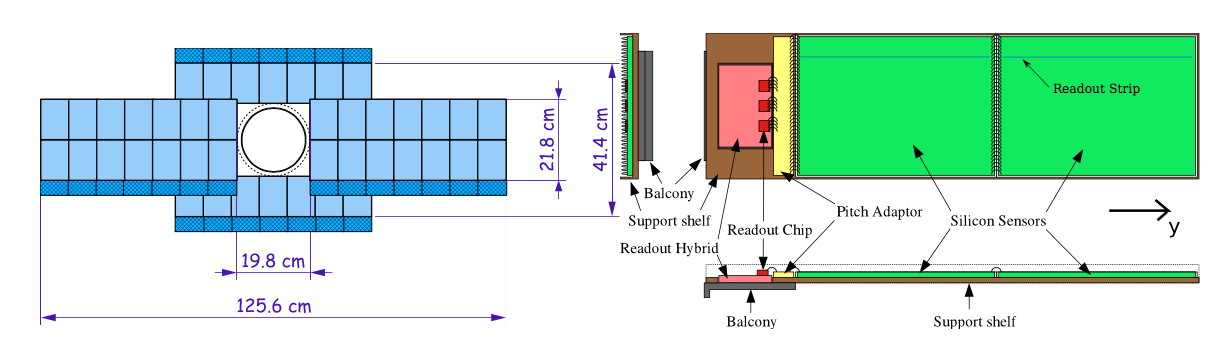
\includegraphics[width=0.9\textwidth]{02LHCb/figs/IT.png}
  \end{center}
  \vspace{-2mm}
  \caption{Schematic view of an IT station (left) and one of the long IT readout modules (right).}
  \label{fig:IT}
\end{figure}

\subsubsection*{The Outer Tracker (OT)}

The OT \cite{LHCb-TDR-006} (Fig.~\ref{fig:OT}) is a gaseous straw-tube detector filled with an Ar/$\rm CO_2$/$\rm O_2$ ($70\%/28.5\%/1.5\%$) gas mixture. It is dedicated to the detection of charged particles in the low track density region outside the IT acceptance and covers a large area of about $340~\rm m^2$. The OT is composed of three stations, where each station has four layers in a X-U-V-X configuration. Each station is separated physically in left and right sides with respect to the beam pipe mounted in support structures called C frames because of their shape. Each layer is divided into two mono-layers. The OT has different types of modules, the long F modules and the short S1, S2, S3 modules that are cut in two pieces to leave space for the IT. The straw tube and anode wire diameters are $5~\rm mm$ and $25~\rm\mu m$ respectively. The hit resolution is about $200~\mu\rm m$.

\begin{figure}[t!]
  \begin{center}
    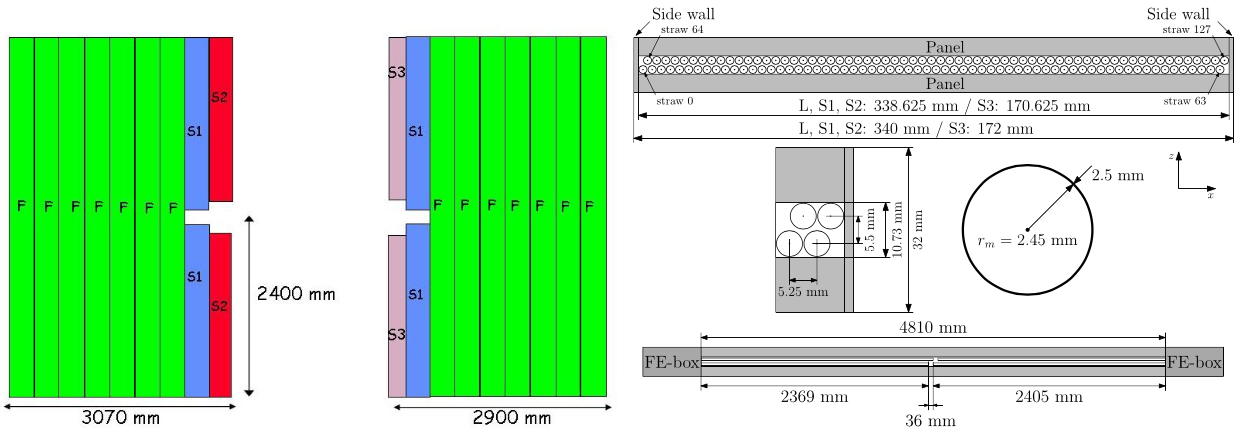
\includegraphics[width=0.9\textwidth]{02LHCb/figs/OT.png}
  \end{center}
  \vspace{-2mm}
  \caption{Schematic view of an OT layer (left) and an OT module layout (right).}
  \label{fig:OT}
\end{figure}

\subsubsection*{Spillover noise in the Silicon Tracker}

Starting from 2015, the time spacing between the LHC proton \emph{bunches} has been $25~\rm ns$, half of the value adopted before. This had a direct impact on the front-end electronics of the silicon detectors (VELO, TT, IT), because the width in time of the analogue signal produced by the front-end electronics is of the same order of magnitude. This means that it is possible to still have a non negligible amount of signal in the subsequent collision, which can be misidentified as coming from particles produced in that event. This source of noise is called \emph{spillover}. The starting seeds of tracking algorithms, called \emph{clusters}, can be polluted by spillover clusters which may increase the number of fake (or \emph{ghost}) reconstructed tracks. 

In the first part of my PhD activity, I studied the effect of splillover clusters in the ST using both simulated events and real collision data. This study shows that this time spacing has little impact on the detector \emph{occupancy}, and that the increase of ghost tracks is negligible. Moreover, it is shown that the charge deposited by particles in the detector can be exploited as a \emph{feature} in multivariate analyses in order to further reduce the ghost track contamination. These results are documented in a note~\cite{spillover} internal to the LHCb collaboration.

\subsection{Particle identification (PID)}
\label{sec:pidintro}

\subsubsection*{The Ring Imaging CHerenkov (RICH) detectors}

When a charged particle is travelling faster than the speed of light in a medium, Cherenkov light is produced at an angle that depends on the velocity of the particle and the refractive index of the medium (\emph{radiator}). By knowing the momentum from the tracker and the velocity from the RICH detectors, the mass can be determined and therefore provide particle identification. Two RICH detectors \cite{RICH} (Fig.~\ref{fig:RICH}) are used in order to provide PID in different momentum ranges.

RICH1 is responsible for providing PID in the momentum range from $1$ to $60\gevc$. The angular acceptance ranges from $25$ to
$50$ ($300$) $\rm mrad$ in the vertical (horizontal) plane. The adopted radiator is fluorobutane ($\rm C_4 F_{10}$). RICH1 is located between the VELO and the TT. 
The Cherenkov photons are guided to Hybrid Photon Detectors (HPD) via dedicated mirrors.

The average kaon identification efficiency in the momentum range from $2$ to $100\gevc$ is $\sim95\%$. The average probability that pions are wrongly identified as kaons is $\sim5\%$ in the same momentum range.

\begin{figure}[t]
  \begin{center}
    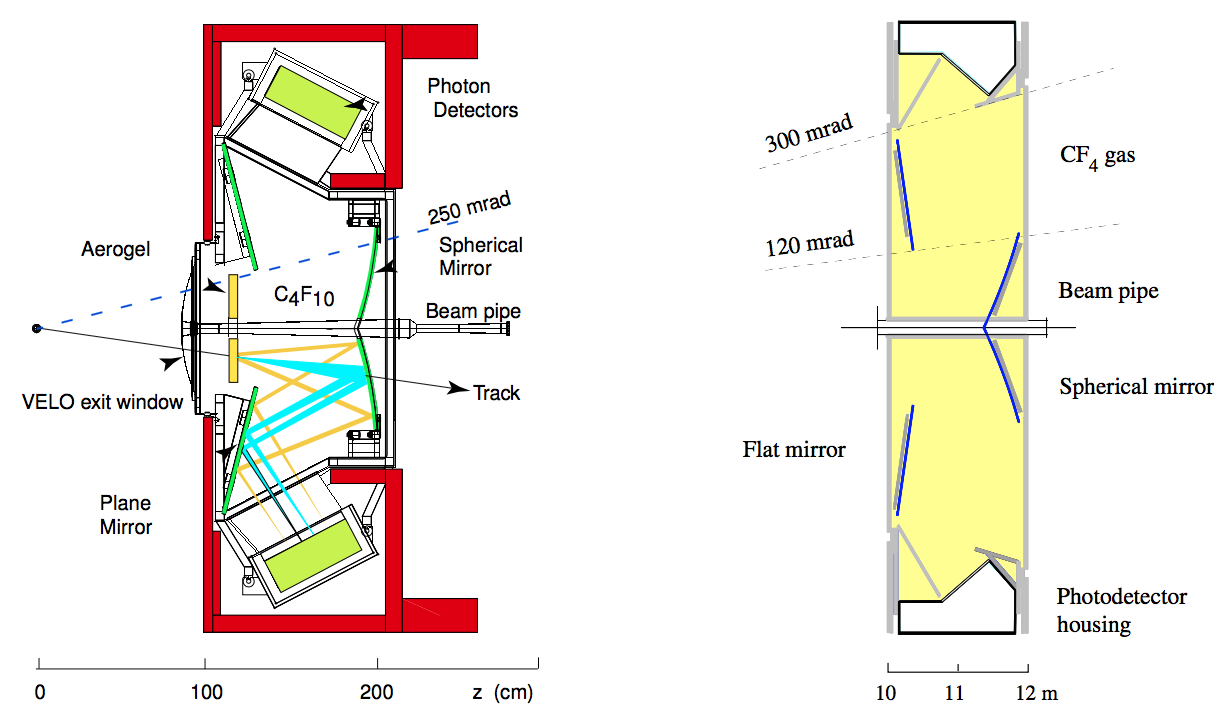
\includegraphics[width=0.8\textwidth]{02LHCb/figs/RICH.png}
  \end{center}
  \vspace{-2.5mm}
  \caption{Side view of RICH1 (left) and top view of RICH2 (right).}
  \label{fig:RICH}
\end{figure}

RICH2 is optimised for the momentum range from $15$ to $100\gevc$. The angular acceptance ranges from $15$ to $100$ ($120$) $\rm mrad$ in the vertical (horizontal) plane where most of the high-momentum tracks are produced. RICH2 uses tetrafluoromethane ($\rm CF_4$) as radiator.

\subsubsection*{The Electromagnetic CALorimeter (ECAL), Pre-Shower (PS) and Scintillator Pad Detector (SPD)}

The ECAL \cite{CAL} is used for the detection and measurement of the energy of electrons and
photons. The ECAL is built as a sandwich of alternating scintillators and
lead layers in the $xy$ plane. Scintillation light produced by the shower of
particles generated by the lead plates is read out by Wave-Length Shifter (WLS) fibres coupled
to PhotoMultiplier Tubes (PMTs). The SPD is installed upstream the ECAL to separate neutral pions
from photons. The PS is installed between the SPD and
the ECAL. Both SPD and PS use scintillator
pads read out by WLS fibres coupled to MultiAnode PhotoMultiplier Tubes (MAPMT). The
acceptance range of the ECAL is from $25$ up to $300$ ($250$) $\rm mrad$ in the horizontal (vertical) 
plane. The relative energy resolution of the ECAL is given by $\sigma_E / E = 10\%/\sqrt{E}\oplus 1\%$, where $E$ is given
in$\gev$.

\subsubsection*{The Hadronic CALorimeter (HCAL)}

The HCAL \cite{CAL} is used for the detection and measurement of the energy of hadrons 
for the first level trigger. A HCAL cell is a sampling device made of
alternating iron and scintillator tiles, where the latter are located along the beam direction. The HCAL
has the same acceptance coverage of the ECAL. The relative energy resolution of the HCAL
is given by $\sigma_E / E = (69\pm 5)\%/\sqrt{E}\oplus (9\pm 2)\%$, where $E$ is given in$\gev$. 

\subsubsection*{Muon detectors}

The muon system \cite{MUON} (Fig.~\ref{fig:MUON}) is a gaseous detector composed of five stations (M1 to M5) interleaved by $80~\rm cm$ thick iron filters. The gaseous detectors are Multi-Wire Proportional Chambers (MWPC), except for the innermost part of M1, where triple Gas Electron Multipliers (GEM) detectors are used to cope with the higher track density. The angular acceptance ranges from $20$ ($16$) to $308$ ($256$) $\rm mrad$ in the horizontal (vertical) plane. The muon detector has $1380$ chambers and covers a total area of $435~\rm m^2$. Each muon chamber is composed of four layers of MPWC, except for M1, where two layers are used. The hit efficiency of the chambers is higher than $99\%$ enabling a trigger efficiency greater than $95\%$ for muons. The adopted gas mixture ($40\%$~Ar, $55\%~\rm CO_2$, $5\%~\rm CF_4$) allows a fast triggering on muons ($40~\rm MHz$).

\begin{figure}[t!]
  \begin{center}
    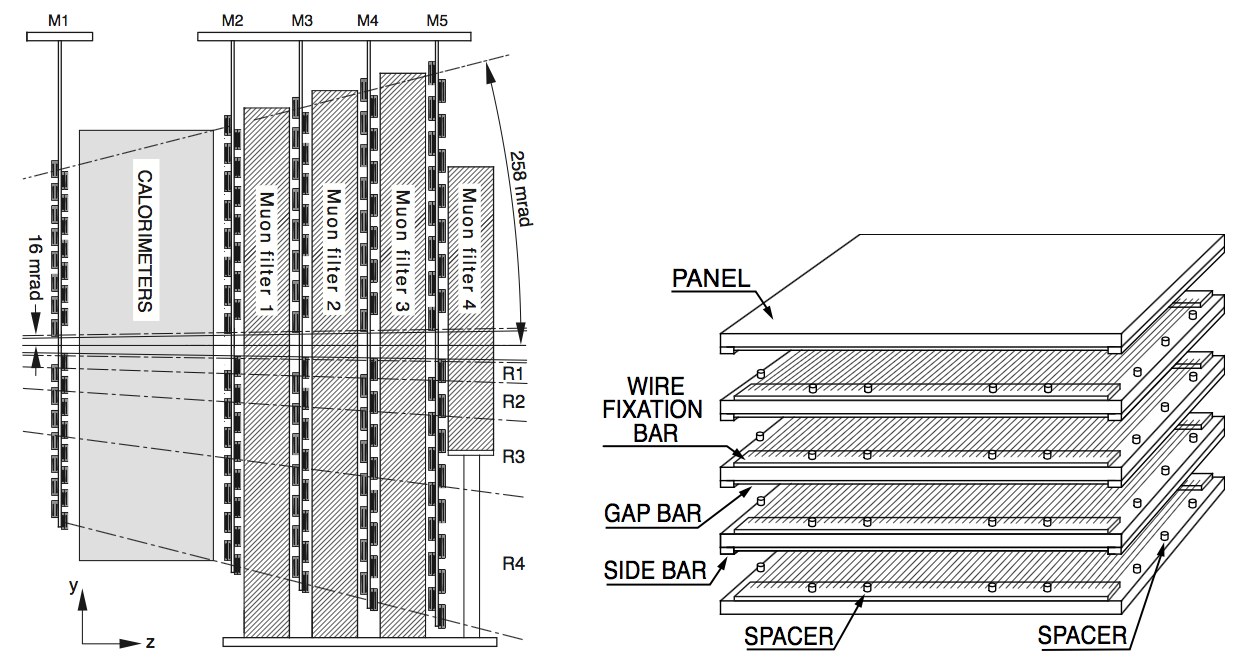
\includegraphics[width=0.9\textwidth]{02LHCb/figs/MUON.png}
  \end{center}
  \vspace{-2mm}
  \caption{Schematic view of the muon system (left) and a MWPC (right).}
  \label{fig:MUON}
\end{figure}

\subsection{Trigger system}

The bunch crossing rate of LHC is very high ($40~\rm MHz$) because more than $99\%$ of the $pp$ collisions do not produce interesting events. It is not possible to record events with such a high rate: therefore, a trigger system \cite{Trigger} is required to reduce the rate from $40~\rm MHz$ down to a few $\rm kHz$. The rate reduction is achieved via selection criteria which ensure that events containing heavy flavour decays are stored. The signatures of these interesting decays include high transverse momentum ($\pt$) and transverse energy ($E_{\rm T}$) of the decay products, as well as displaced decay vertices 
or tracks with large impact parameter (IP) with respect to the $pp$ collision point due to the relative long lifetimes of $b$ and $c$ hadrons. The trigger is divided into two sequential stages: a hardware stage called Level-0 (L0) trigger, and a software stage called High Level Trigger (HLT). Different trigger decisions are separated into various \emph{lines}, each of which provides information on different physics processes (\eg~decay topology, presence of muons etc\dots). All the trigger steps are summarised in Fig.~\ref{fig:trigger}.

Two types of trigger response are assigned offline, when some physics channel is analysed. The TOS (\emph{Trigger On Signal}) trigger occurs when the presence of the signal is sufficient to have a positive trigger decision. The TIS (\emph{Trigger Independent of Signal}) trigger occurs when, after removing signal tracks and hits associated to them, another signature in the event is sufficient to have a positive trigger decision.

After the trigger stage, the data go through further offline selection steps, where exclusive (\eg~$\Bz\to \Dmp\pipm$, $\Bpm\to J/\psi K^{\pm}$) and inclusive (\eg~$b$~hadron~$\to J/\psi X$, $J/\psi\to\mu^+\mu^-$) decays are reconstructed at higher quality than was possible in the strict timing requirements of the trigger, and further selections are applied.
This offline selection step is known as \emph{stripping}, and each set of selection requirements is called \emph{stripping line}.

\begin{figure}[htbp]
  \begin{center}
    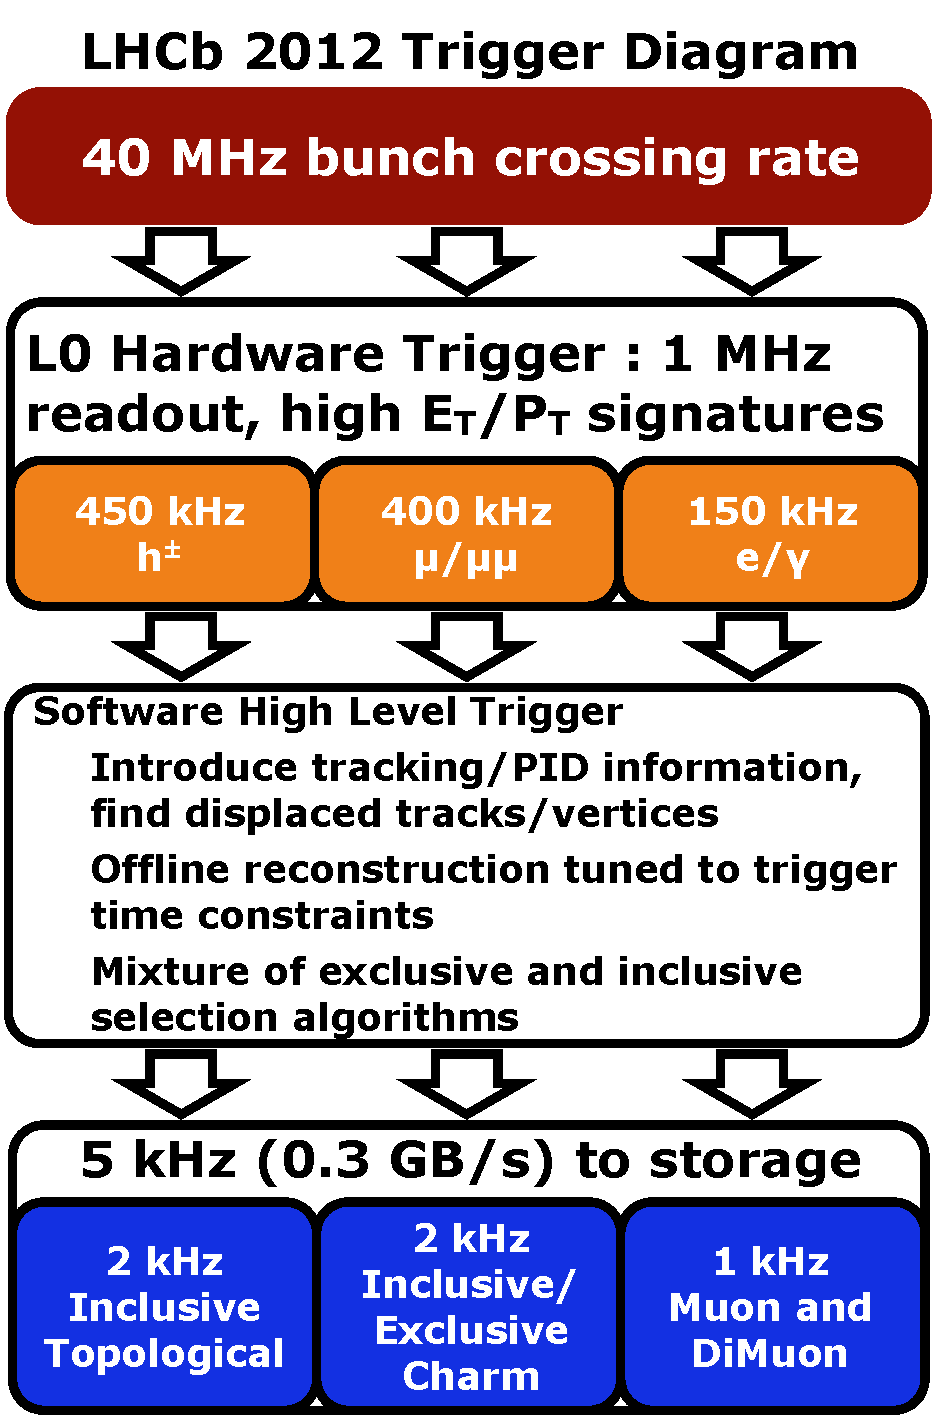
\includegraphics[width=0.45\textwidth]{02LHCb/figs/TriggerRunI.pdf}
    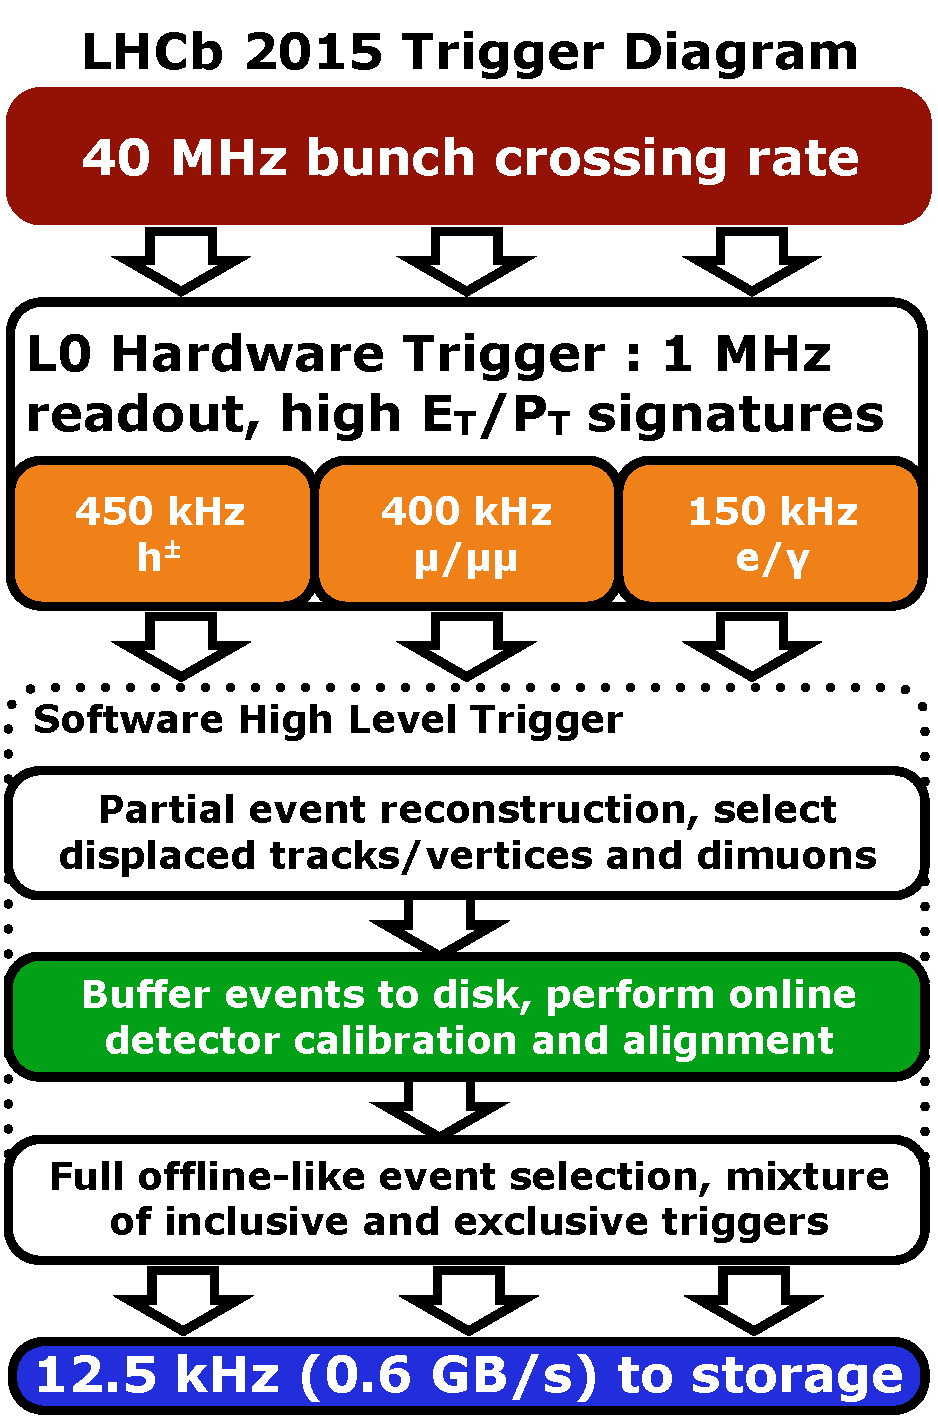
\includegraphics[width=0.45\textwidth]{02LHCb/figs/TriggerRunII.pdf}
  \end{center}
  \vspace{-2mm}
  \caption{Summary of the trigger strategies followed during the Run 1 (2011--2012, left) and Run 2 (2015--2017, right) data-taking periods. During Run 2, an online detector and calibration alignment was introduced, as well as full event selections (both inclusive and exclusive).}
  \label{fig:trigger}
\end{figure}

\subsubsection*{Level-0 trigger (L0)}

The L0 mainly exploits the calorimeters and muon chambers. The idea behind the L0 is to select events that contain high \pt~muons and high $E_{\rm T}$ hadrons, electrons and photons, which very likely come from $b$- and $c$-hadron decays, by using simple signatures that do not require the reconstruction of the event.
The L0 reduces the data rate from $40~\rm MHz$ down to $1~\rm MHz$, which is the rate limit of the LHCb readout electronics.

\subsubsection*{High Level Trigger (HLT)}

The HLT is separated into two stages, HLT1 and HLT2, and runs on about $29\,000$ commercial CPU cores. 

At the HLT1 level, the full detector information is read out, and then track/vertex reconstruction and PID are performed. The exploited signatures are mainly the presence of high \pt~tracks, high transverse energy calorimeter clusters (photons and $\pi^0$), high invariant mass of muon pairs, and tracks with large IP. All the HLT1 trigger lines are \emph{inclusive}, meaning that only decay products common to various decay processes are selected rather than specific decays. After the HLT1, the rate goes down to about $70~\rm kHz$.

The HLT2 is a combination of inclusive selections and algorithms that reconstruct entirely (\emph{exclusively}) some decay processes. The main lines are topological lines using Multi-Variate Analysis (MVA) techniques with different sets of kinematic and position features as input, exclusive charm lines and high mass displaced di-hadron/lepton lines. After the HLT2, the events are stored on tape for further offline analysis.

\subsection{Event reconstruction and simulation}

\subsubsection*{Track and vertex reconstruction}

Starting from the \emph{hits} in the tracking detectors, tracks and vertices are reconstructed via dedicated algorithms. 
Different track types are reconstructed, as shown in Fig.~\ref{fig:trackTypes}. Each track is characterised by hits collected in different sub-detectors. For example, downstream tracks, with no hits in the VELO,
are typically associated to long-lived particles such as $\Lambda$ and $K^0_{\rm S}$. Because of the vertical magnetic field, tracks are bend in the $xz$ plane. By knowing the reconstructed particle trajectory and 
the magnetic field map, it is possible to measure the momentum of the particle.

\begin{figure}[htbp]
  \begin{center}
    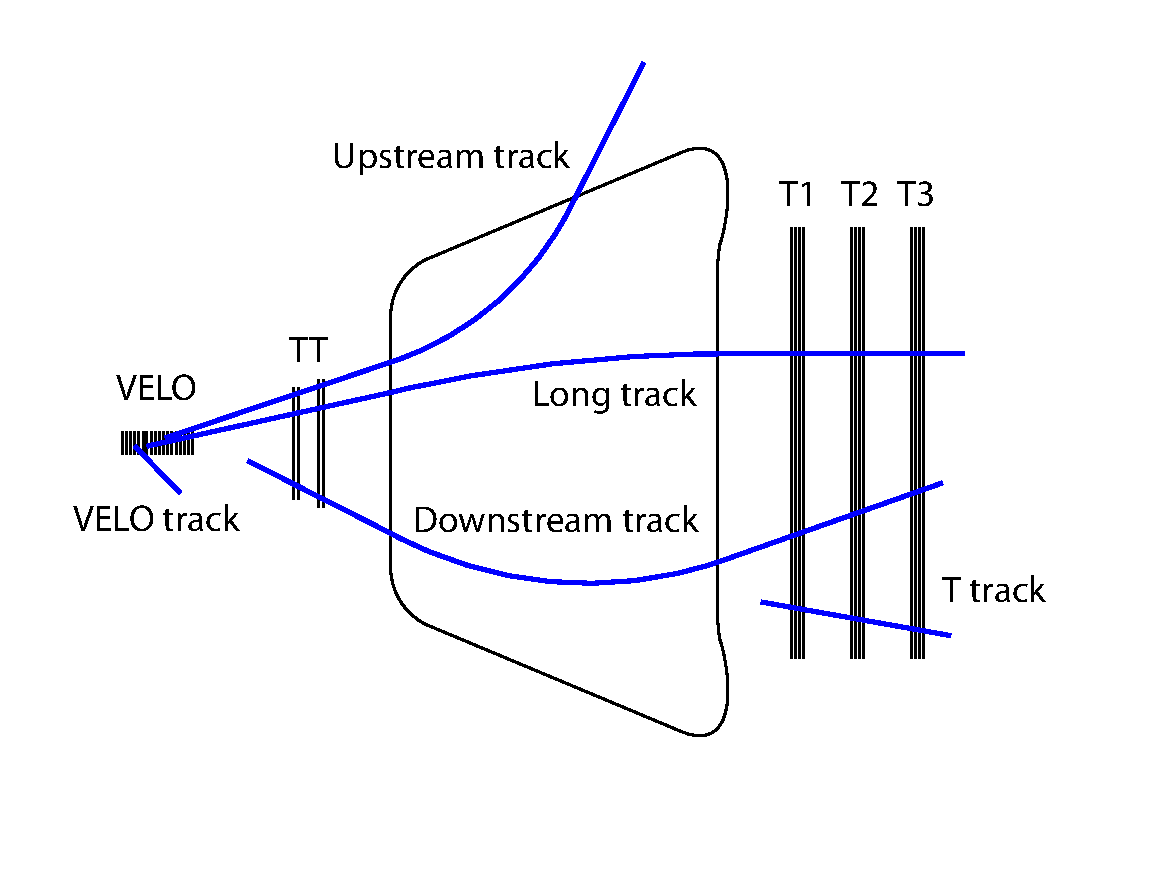
\includegraphics[width=0.9\textwidth]{02LHCb/figs/trackTypes.pdf}
  \end{center}
  \vspace{-15mm}
  \caption{Schematic description of the different track types reconstructed in LHCb.}
  \label{fig:trackTypes}
\end{figure}

\subsubsection*{PID}
The Cherenkov radiation emitted by charged particles in the RICH radiators produces \emph{rings} in the RICH acceptance, which are reconstructed via pattern recognition algorithms.
For each reconstructed pattern, the \emph{likelihood} $\mathcal L_{\pi}$ for the ring to be produced by a pion (the most common particle in the LHCb environment) is computed.
The momentum of the particle is also used in the likelihood computation.
Then, likelihood functions for other hypotheses (kaon, proton, electron, muon) are computed and compared with the pion likelihood.
For a given particle X (X=$e,\mu,p,K$), the PIDX observable is defined as
\begin{equation}
	\label{eq:pidx}
	\rm PIDX = \ln \mathcal L_{\rm X} - \ln \mathcal L_{\pi}.
\end{equation}
In typical LHCb analyses, requirements on the PID observables are applied to suppress physical backgrounds due to wrongly-identified particles.
The PID observables are adopted, together with other kinematic and detector-related observables, as input feature for neural networks which predict the probability for a
particle to be either an electron, a muon, a proton, a kaon, or a pion. This probability is denoted as PROBNNX (X=$e,\mu,p,K,\pi$).

\subsubsection*{Simulation}
The Monte Carlo (MC) simulation of $pp$ collisions, particle decays, and interactions with the detector are crucial in the validation of physics analyses.
The parton-parton collision and hadronisation simulation is performed by \texttt{PYTHIA}~\cite{Sjostrand:2007gs}, interfaced to \texttt{EvtGen}~\cite{Lange:2001uf} for the decay of the hadrons and leptons for standard productions. The QED corrections to the decay (\ie~the emission of radiation photons) is generated by the \texttt{PHOTOS} package~\cite{Golonka:2005pn}. The interactions of particles with the detector material and their tracking in the magnetic field are simulated by \texttt{GEANT4}~\cite{Agostinelli:2002hh,Allison:2006ve}.

\subsection{Data collected by LHCb}
\label{sec:lhcdata}

The collision rate $R$ $[\rm s^{-1}]$ in LHC can be expressed in terms of the \emph{cross-section} $\sigma$ $[\rm cm^2]$ and the \emph{luminosity} $\mathcal L$ $[\rm s^{-1} \rm cm^{-2}]$ as
\begin{equation}
	R = \mathcal L \sigma.
\end{equation}
For a given data-taking period, the \emph{integrated luminosity} $L~[\rm cm^{-2}]$ is a measure of the amount of recorded data. The typical unit for luminosity is the inverse \emph{barn}, which corresponds to $10^{24}~\rm cm^{-2}$. The LHCb integrated luminosity is of the order of an inverse \emph{femtobarn} ($\rm fb^{-1}$); one inverse femtobarn corresponds to the production of about $10^{11}$ $b\bar b$ quark pairs. 

The LHCb detector collected data produced mainly from $pp$ collisions in the 2010--2017 period, so far. During the 2011--2012 data-taking period, called \emph{Run 1}, about $3\rm~fb^{-1}$ of data were collected. The centre-of-mass energy $\sqrt{s}$ of the $pp$ interactions was $7~\rm TeV$ and $8~\rm TeV$ in 2011 and 2012, respectively, and the time spacing between \emph{bunches} of protons in the LHC was $50~\rm ns$.
The 2013--2014 period, known as \emph{Long Shutdown 1} (LS1), was dedicated to work on the LHC machine to bring the energy up.
The \emph{Run 2} data-taking period started in 2015, and is planned to last until the end of 2018. The centre-of-mass energy of the $pp$ collisions during Run 2 is $13~\rm TeV$, whereas the time spacing between proton bunches is $25~\rm ns$. In the 2015--2017 data taking period, about $3.7~\rm fb^{-1}$ of data were collected. The data collected during each year is summarised in Fig.~\ref{fig:luminosity}.

\begin{figure}[htbp]
  \begin{center}
    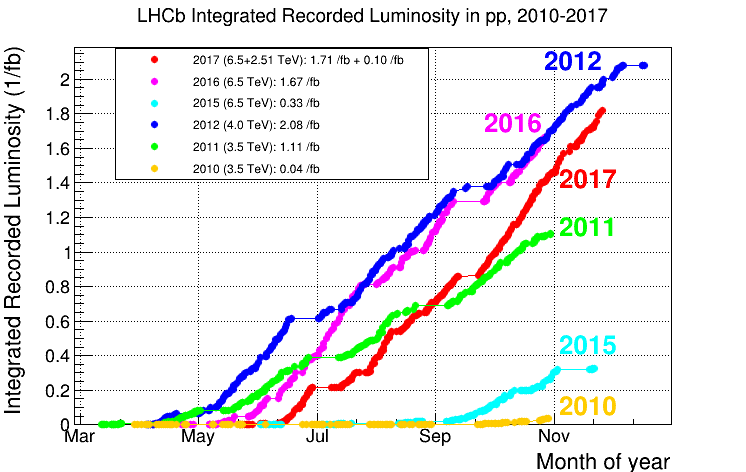
\includegraphics[width=0.9\textwidth]{02LHCb/figs/Luminosity.png}
  \end{center}
  \vspace{-2mm}
  \caption{Integrated luminosity of $pp$ collisions collected each year by LHCb.}
  \label{fig:luminosity}
\end{figure} 
